\documentclass[a4paper,10pt]{article}
\usepackage[utf8]{inputenc}
\usepackage{amsmath}
\usepackage{amsfonts}
\usepackage{amssymb}
\usepackage{algorithm}
\usepackage[noend]{algpseudocode}
\usepackage{program}
\usepackage{amsmath}
\usepackage{graphicx}
\usepackage[T1]{fontenc}
\usepackage{eso-pic}
%\usepackage{gensymb}
\usepackage{listings}
\usepackage{float}
\usepackage{hyperref}
\usepackage{su17}

\usepackage{xcolor}
\definecolor{alternateKeywordsColor}{rgb}{0.13,1,0.13}
\definecolor{keywordsColor}{rgb}{0.13,0.13,1}
%\definecolor{commentsColor}{rgb}{0,0.5,0}
\definecolor{commentsColor}{rgb}{0,0.5,0}
%\definecolor{stringsColor}{rgb}{0.9,0,0}
\definecolor{stringsColor}{rgb}{0,0,0.5}
\definecolor{light-gray}{gray}{0.95}

\hypersetup{
    colorlinks=true,
    linkcolor=blue,
    filecolor=magenta,      
    urlcolor=cyan,
}
 
\urlstyle{same}

\newcommand\floor[1]{\lfloor#1\rfloor}
\newcommand\ceil[1]{\lceil#1\rceil}
\newcommand{\BackgroundPic}{\put(-4,0){\parbox[b][\paperheight]{\paperwidth}{\centering\includegraphics[width=\paperwidth,height=\paperheight]{nat-farve.pdf}}}}

\algnewcommand\True{\textbf{true}\space}
\algnewcommand\False{\textbf{false}\space}
\algdef{SE}[SUBALG]{Indent}{EndIndent}{}{\algorithmicend\ }%
\algtext*{Indent}
\algtext*{EndIndent}

\lstdefinelanguage{console}{%
  keywords={},
  morekeywords={},
  otherkeywords={},
  basicstyle=\ttfamily\lst@ifdisplaystyle\small\fi, 
  breaklines=true,
  showstringspaces=false,
  % aboveskip=0pt, 
  % belowskip=0pt,
  %resetmargins=true,
  captionpos=b,
  backgroundcolor=\color{green!10!white},
}


\header{%
  assignment={Exercise Set 0: Geometrical Objects},%
  authors={Adam Frederik Ingwersen Linnemann <\texttt{gqr701@alumni.ku.dk}>},%
  shortAuthors={\texttt{gqr701}},%
  date={Friday, February 10, 15:00}
}

\begin{document}
	\AddToShipoutPicture*{\BackgroundPic}
	
	\begin{titlepage}
		\thispagestyle{empty}
		\vspace*{5cm}
		\begin{center}
			\Huge \textbf{ Software Udvikling } \\
			\LARGE \textbf{Exercise Set 0: Geometrical Objects} \\
		\end{center}
		\vspace*{3.5cm}
		\begin{flushleft}
			
		\begin{table}[h!]
			\begin{tabular}{lll}
				Adam Ingwersen\\
		\end{table}
			
			
			\vspace{3mm}
			\vspace{3mm}
			Datalogisk  Institut\\
			Københavns Universitet\\
			\vspace{3mm}
			\today\\
			%\vspace*{0.5cm}
			
		\end{flushleft}
	\end{titlepage}

	\title{***}
	\author{***}
	
	\newpage
\newpage

\section*{Introduktion}
Denne afleveringsopgave har til formål at gennemgå basale OOP-koncepter, C\# samt IDE'et \texttt{Monodevelop}. 

\section{Install Party}
Completed.

\section{Geometry}
\subsection{Console Project}

\begin{figure}[H]
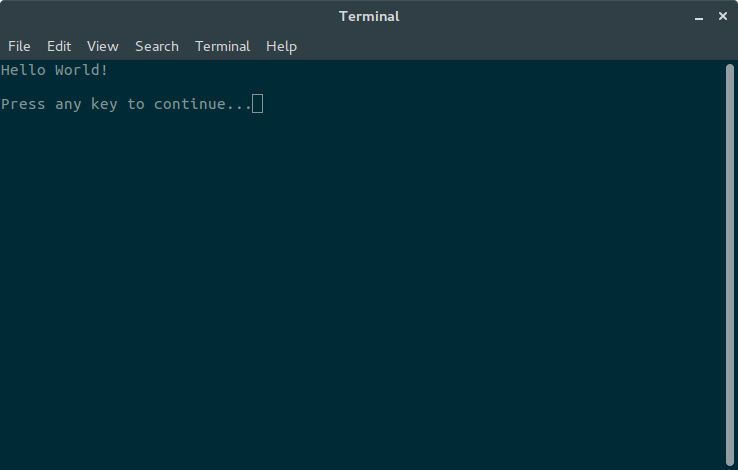
\includegraphics[width=\textwidth]{Screenshots/hello.png}
    \centering
    \caption{Output af Run Item}
    \label{fig:my_label}
\end{figure}


\subsubsection*{2.7}
\begin{enumerate}
  \item What is "Hello World!"?
  \begin{enumerate}
    \item "Hello World!" er beskeden, der printes til konsollen via \textbf{System.Console.WriteLine}-funktionen.
  \end{enumerate}
  \item What is \textbf{Console.WriteLine}?
  \begin{enumerate}
    \item En funktion, der tilhører \textbf{System.Console namespacet}. Denne printer en string til konsollen.
  \end{enumerate}
  \item What is \textbf{Main}?
  \begin{enumerate}
    \item \textbf{Main()} er en method. En C# applikation begynder eksekveringen efter kald til \textbf{Main()}.
  \end{enumerate}
  \item What is \textbf{MainClass}?
  \begin{enumerate}
    \item Dette er navnet på en klasse, der indeholder \textbf{Main()}-metoden. Navnet er underordnet, men bør jf. kodestandarden, have uppercase forbogstav.
  \end{enumerate}
  \item What is \textbf{HelloWorld}?
  \begin{enumerate}
    \item Det nye navn på klassen, der indeholder \textbf{Main()}-metoden. Hvis programmet køres uden \texttt{using System;}, som er namespace-deklarationen, fås en fejl. Dette er fordi, C# ikke kan finde en funktion \textbf{Console.WriteLine} uden \textbf{System}. 
  \end{enumerate}
  \item What are \textbf{args}?
  \begin{enumerate}
    \item En argument-deklaration eller \textbf{constructor}.
  \end{enumerate}
  \item What is \textbf{System}?
  \begin{enumerate}
    \item System er en namespace, med en række funktioner, herunder \textbf{Console}.
  \end{enumerate}
  \item What are \textbf{Console}?
  \begin{enumerate}
    \item Se ovenfor.
  \end{enumerate}
\end{enumerate}

\subsection{Library Project}

Der er i den nye udgave af \texttt{Monodevelop} intet, der hedder \textbf{Refactor}. 

Efter at have lavet nyt Library Project, og refereret til det nye library i Main ved at tilføje:

\begin{minted}
{csharp}
Vertex test = new Vertex ();
Console.WriteLine (test);
\end{minted}

Fås følgende output: 
\begin{figure}[H]
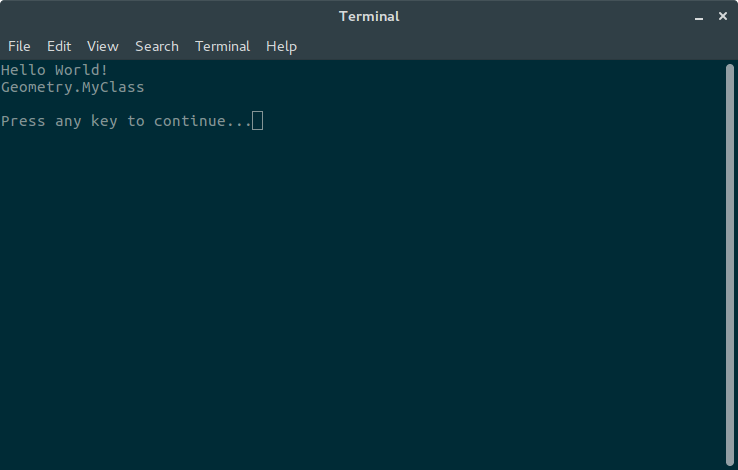
\includegraphics[width=\textwidth]{Screenshots/hello2.png}
    \centering
    \caption{Tilføjelse af Vertex()}
    \label{fig:my_label}
\end{figure}

Her ses det, at det refererede objekt bliver skrevet til konsollen som en string. 

\subsection{Gtk# 2.0 Project}

Denne del fungerede efter hensigten.

\begin{figure}[H]
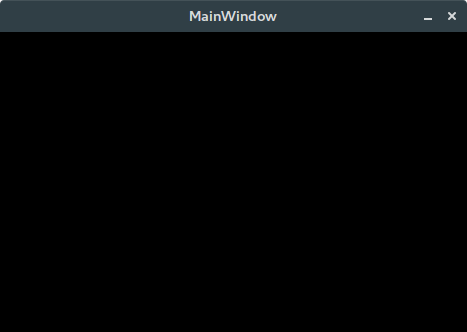
\includegraphics[width=\textwidth]{Screenshots/mainwindow.png}
    \centering
    \caption{Sort MainWindow}
    \label{fig:my_label}
\end{figure}

\section{Geomtery II}

\subsection{Vertex}

Her defineres et struct som et punkt besteående af to integers og overrider \textbf{ToString()}-funktionen.

\begin{minted}
{csharp}
public struct Vertex
{
    public int x, y;
    public Vertex(int x, int y)
    {
        this.x = x;
        this.y = y;
    }
    public override string ToString()
    {
        return(String.Format("({0},{1})", x, y));
    }
}
\end{minted}

For at undersøge, hvorvidt dette fungerer efter intentionen, instantieres klassen med input til konstruktoren;

\begin{minted}
{csharp}
Vertex test = new Vertex(1,2);
\end{minted}

Ved udskrift fås det ønskede output:

\begin{figure}[H]
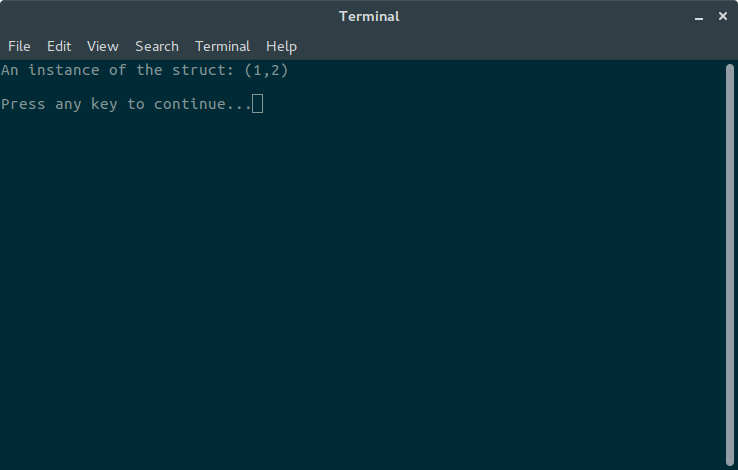
\includegraphics[width=\textwidth]{Screenshots/struct.png}
    \centering
    \caption{Test: ToString override}
    \label{fig:my_label}
\end{figure}

Hereffter, kan operatorerne $==$ og $!=$ overloades for Vertex på følgende måde.

\begin{minted}
{csharp}
public static bool operator ==(Vertex l, Vertex r)
{
    return Equals(l, r);
}

public static bool operator !=(Vertex l, Vertex r)
{
    return !Equals(l, r);
}
\end{minted}

Funktionaliteten testes i TUI-projektet ved: 
\newline
\begin{minted}
{csharp}
Vertex a = new Vertex(1, 1);
Vertex b = new Vertex(2, 1);

Console.WriteLine ("a == b : {0}", a == b);
Console.WriteLine ("a == a : {0}", a == a);
Console.WriteLine ("a != a : {0}",a != a);
Console.WriteLine ("a != b : {0}",a != b);
\end{minted}

Ved kørsel skrives det ønskede output til konsollen:

\begin{figure}[H]
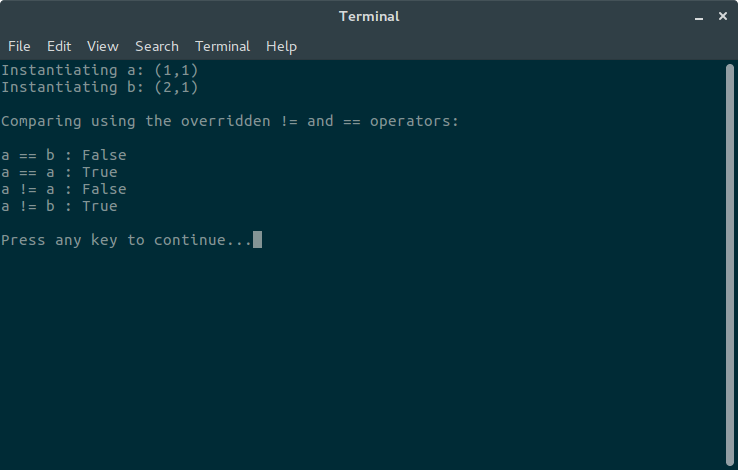
\includegraphics[width=\textwidth]{Screenshots/bool.png}
    \centering
    \caption{Test: Boolean override}
    \label{fig:my_label}
\end{figure}
\newline

Det bemærkes her, at der kommer en advarsels-prompt i IDE'et; \texttt{"A comparison made to same variable. Did you mean to compare something else?"}. Denne advarsel forekommer ufarlig, eftersom den advarer mod netop det, der ønskedes afprøvet.

For at override \textbf{Equals()}-operatoren, bemærkes det, at denne skal kunne håndtere objekter - udover værdier, som de foregående operatorer. Denne løsning bygger på de to foregående operatorer:

\begin{minted}
{csharp}
public override bool Equals(Object struc) 
{
    if (struc == null || GetType() != struc.GetType()) 
        return false;
    Vertex p = (Vertex)struc;
    return (x == p.x) && (y == p.y);
}
\end{minted}


Løsningen fungerer efter hensigten:

\begin{figure}[H]
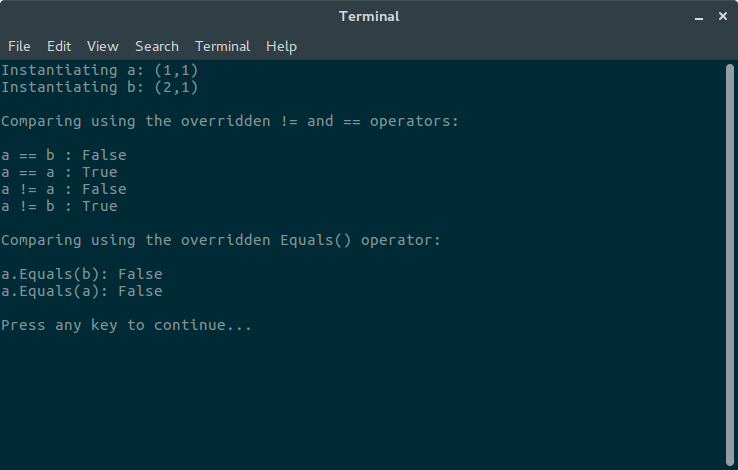
\includegraphics[width=\textwidth]{Screenshots/equals.png}
    \centering
    \caption{Test: Equals() override}
    \label{fig:my_label}
\end{figure}
\newline

Denne delopgave er ikke færdiggjort. 

\subsection{Polygons}
TBA

\section{Testing}

Denne delopgave er ikke påbegyndt.

\section{Getting started with the LATEX Template}

Jeg får uhenigtsmæssige farver, de steder, hvor \texttt{minted} er anvendt. C\#-koden er derfor ikke pænt præsenteret. 

\end{document}